%%%%%%%%%%%%  JJCIT-latex Template  %%%%%%%%%%%%%%

\documentclass[11pt,twoside]{articleJJCIT}
\usepackage{amsmath}
\usepackage{latexsym}
\usepackage{amsfonts}
\usepackage{caption}

%\usepackage{natbib}
\usepackage[square,sort,comma,numbers]{natbib}
\usepackage[normalem]{ulem}
\usepackage{array}
%\usepackage{cuted}
\usepackage{amssymb}
\usepackage{graphicx}
%\pagestyle{fancy}
\usepackage{secdot}
%\sectiondot{subsection}
\usepackage{times}
\usepackage{mathptmx}
\usepackage[T1]{fontenc}
\usepackage{lmodern}
\usepackage{garamond}
\usepackage{subfig}
\usepackage{wrapfig}
\usepackage{wasysym}
\usepackage{enumitem}
\usepackage{adjustbox}
\usepackage{ragged2e}
\usepackage[svgnames,table]{xcolor}
\usepackage{tikz}
\usepackage{longtable}
\usepackage{changepage}
\usepackage{setspace}
\usepackage{hhline}
\usepackage{multicol}
\usepackage{tabto}
\usepackage{float}
\usepackage{multirow}
\usepackage{makecell}
\usepackage{fancyhdr}
\usepackage[toc,page]{appendix}
\usepackage[hidelinks]{hyperref}
\usetikzlibrary{shapes.symbols,shapes.geometric,shadows,arrows.meta}
\tikzset{>={Latex[width=1.5mm,length=2mm]}}
\usepackage{flowchart}\usepackage[paperheight=11.69in,paperwidth=8.27in,left=0.98in,right=0.98in,top=0.98in,bottom=0.59in,headheight=1in]{geometry}
\usepackage[utf8]{inputenc}
\usepackage[T1]{fontenc}
\TabPositions{0.5in,1.0in,1.5in,2.0in,2.5in,3.0in,3.5in,4.0in,4.5in,5.0in,5.5in,6.0in,}
\urlstyle{same}
\setcounter{tocdepth}{5}
\setcounter{secnumdepth}{5}




%%%%%%%%%%%%  Set Depths for Nested Lists created by \begin{enumerate} \setlistdepth{9}
\renewlist{enumerate}{enumerate}{9}
		\setlist[enumerate,1]{label=\arabic*)}
		\setlist[enumerate,2]{label=\alph*)}
		\setlist[enumerate,3]{label=(\roman*)}
		\setlist[enumerate,4]{label=(\arabic*)}
		\setlist[enumerate,5]{label=(\Alph*)}
		\setlist[enumerate,6]{label=(\Roman*)}
		\setlist[enumerate,7]{label=\arabic*}
		\setlist[enumerate,8]{label=\alph*}
		\setlist[enumerate,9]{label=\roman*}
\renewlist{itemize}{itemize}{9}
		\setlist[itemize]{label=$\cdot$}
		\setlist[itemize,1]{label=\textbullet}
		\setlist[itemize,2]{label=$\circ$}
		\setlist[itemize,3]{label=$\ast$}
		\setlist[itemize,4]{label=$\dagger$}
		\setlist[itemize,5]{label=$\triangleright$}
		\setlist[itemize,6]{label=$\bigstar$}
		\setlist[itemize,7]{label=$\blacklozenge$}
		\setlist[itemize,8]{label=$\prime$}
\pagenumbering{gobble}
\date{}
 %%%%%%%%%%%%  Header here  %%%%%%%%%%%%%%
\pagestyle{fancy}
\fancyhf{}
\fancyhead[LE]{\thepage{\fontsize{8pt}{11pt}\selectfont "How To Prepare Paper Manuscript for Possible Publication in JJCIT", A. Jones and G. Filtman.}}
\fancyhead[LO]{ {\fontsize{8pt}{11pt}\selectfont Jordanian Journal of Computers and Information Technology (JJCIT), Vol. X, No. X.}}
{\fontsize{8pt}{11.0pt}\selectfont}\renewcommand{\headrulewidth}{0pt}
\setlength{\topsep}{0pt}\setlength{\parindent}{0pt}
%\renewcommand{\arraystretch}{1.3}
%\ExecuteOptions{roman}

%%%%%%%%%%%%%%%%%%%% Document code starts here 
\begin{document}
%Title goes here%%%%%%%%%%%%%%%%%%%%
%\uppercase 
\title{\fontsize{20pt}{11.0pt} \textbf{HOW TO PREPARE YOUR PAPER MANUSCRIPT FOR POSSIBLE PUBLICATION IN JJCIT}}
\setlength{\parskip}{12.0pt}\par
%\thispagestyle{fancy} 
%\setlength{\parskip}{0pt}
%Authors go here%%%%%%%%%%%%%%%%%%%%
\author{Adam Johns\footnote{A. Jones is with Department of Computer Engineering, Big University, City, Country. Email: a.johns@xx.yy.zz} and George Filtman\footnote{G. Filtman is with Exceptional Software, New Street, City, Country. Email: g.filtman@zzz.com}}
\maketitle
%\setlength{\parskip}{18.0pt}

{\fontsize{13pt}{11pt} \textit{\textbf{ABSTRACT}}}
\setlength{\parskip}{12.0pt}\par
\fontsize{10pt}{11.0pt}\selectfont 
%%%%%%%%%%ABSTRACT goes here%%%%%%%%%%%
{\textit{This paper gives complete guidelines for authors submitting papers for the JJCIT.}}\par
%%%%%%%%%%KEYWORDS%%%%%%%%%%%
{\fontsize{13pt}{10pt} \textit{\textbf{KEYWORDS}}}\par
\setlength{\parskip}{12.0pt}
{\textit{Mobile Telecommunications, Network Protocols, Wireless Network, Mobile Network.}}


\section{Introduction}
This document describes, and is written to conform to, author guidelines for Jordanian Journal of Computers and Information Technology (JJCIT). It is prepared in Microsoft Word as a .doc document. It is the only acceptable means of preparing manuscripts. Final camera-ready versions must conform to this layout too. Microsoft\ Word terminology is used where appropriate in this document.  Although formatting instructions may often appear daunting, the simplest approach is to use this template and insert headings and text into it as appropriate.\par

\section{Format Guide}
The following formatting rules must be followed strictly. This (.doc) document may be used as a template for papers prepared using Microsoft Word. Papers not conforming to these requirements may not be published in JJCIT.

\subsection{General Format, Page Layout and Margins}

Standard A4 (210mm x 297mm) portrait page set-up should be used.  The left, right, top margins should be 25mm and bottom margins should be 15mm. Do not use any headers, footers or footnotes.  No page numbers. Single column.  All main text paragraphs, including the abstract, must be fully (left and right) justified.  All text, including title, authors, headings, captions and body, will be Times New Roman font.

%\setlength{\parskip}{6.0pt}
\subsection{Title}
%\setlength{\parskip}{12.0pt}
The title is to be written in 20 pt. Garamond font, centred and using the bold and $``$Capital\ Caps$"$  formats.  There should be 18 pt. (paragraph) spacing after the last line.

%\setlength{\parskip}{6.0pt}
%\setlength{\parskip}{12.0pt}
\subsection{Authors}

Author names are to be written in 13 pt. Times New Roman format, centred and followed by a 18 pt.\ paragraph\ spacing.  If necessary, use superscripts to link individual authors with institutions as shown above. Author affiliations are to be written in 12 pt. Times New Roman, centred, with email addresses, in 10 pt. Courier New, on the line following. The last email address will have an 18 pt. (paragraph) spacing following.

\subsection{Abstract}
The Abstract section begins with the word, ``Abstract"  in 13 pt. Times New Roman, bold italics, ``Capital Caps" font with a 6pt. spacing following.  The abstract must not exceed 150 words in length in 10 pt. Times New Roman italics.  The text must be fully justified, with a 12 pt. paragraph spacing following the last line.

\subsection{Keywords}
 The Keywords section begins with the word, $``$Keywords$"$  in 13 pt. Times New Roman, bold italics, $``$Capital\ Caps$"$ \ font with a 6pt. spacing following.  There may be up to five keywords (or short phrases) separated by commas and six spaces, in 10 pt. Times New Roman italics.  An 18 pt. line spacing follows.

\subsection{Section and Sub-Section Headings}
Section headings are numbered 1. Xxx, 2. Yyy, etc. in 14 pt. bold $``$Small Caps$"$  Times New Roman font with a 6 pt. line spacing following. 

Subsection headings are numbered 1.1. Aaa, 1.2. Bbb, etc. in 12 pt. bold Times New Roman font with a 6pt line spacing following.

\subsubsection{Further Subsections}

 Further sub-sectioning, if required, is indicated using 1.1.1. Qqq, etc. headings with 11 pt. bold Times New Roman font with a 6pt line spacing following.
 
\subsection{Text}
Main-body text is to written in fully (left and right) justified 11 pt. Times New Roman font with a 6pt. (paragraph) line spacing following the last line of each paragraph, but a 12pt. (paragraph) line spacing following the last paragraph. Do not indent paragraphs.

\subsection{Figures and Tables}
 

%%%%%%%%%%%%%%%%%%%% Table No: 1 starts here %%%%%%%%%%%%%%%%%%%%
{\fontsize{11pt}{12pt}
{\setlength\extrarowheight{3pt}
\begin{longtable}{p{1.12in}p{0.92in}p{2.05in}p{1.16in}}
\caption{Heading and text fonts.}
\endfirsthead
\multicolumn{4}{c}{\textit{}}
\endhead\hline
\multicolumn{4}{r}{\textit{}} \\
\endfoot
\hline 
\endlastfoot\hline
%row no:1
\multicolumn{1}{|p{1.12in}}{{\fontsize{11pt}{13.2pt}\selectfont \textbf{Text}}} & 
\multicolumn{1}{|p{0.92in}}{{\fontsize{11pt}{13.2pt}\selectfont \textbf{Alignment}}} & 
\multicolumn{1}{|p{2.05in}}{{\fontsize{11pt}{13.2pt}\selectfont \textbf{Font}}} & 
\multicolumn{1}{|p{1.16in}|}{{\fontsize{11pt}{13.2pt}\selectfont \textbf{Followed by:}}} \\
\hhline{----}
%row no:2
\multicolumn{1}{|p{1.12in}}{{\fontsize{11pt}{13.2pt}\selectfont Title}} & 
\multicolumn{1}{|p{0.92in}}{{\fontsize{11pt}{13.2pt}\selectfont Centre}} & 
\multicolumn{1}{|p{2.05in}}{{\fontsize{11pt}{13.2pt}\selectfont 20 pt. TNR, bold, capital-caps}} & 
\multicolumn{1}{|p{1.16in}|}{{\fontsize{11pt}{13.2pt}\selectfont 24 pt. line sp.}} \\
\hhline{----}
%row no:3
\multicolumn{1}{|p{1.12in}}{{\fontsize{11pt}{13.2pt}\selectfont Authors}} & 
\multicolumn{1}{|p{0.92in}}{{\fontsize{11pt}{13.2pt}\selectfont Centre}} & 
\multicolumn{1}{|p{2.05in}}{{\fontsize{11pt}{13.2pt}\selectfont 13 pt. TNR }} & 
\multicolumn{1}{|p{1.16in}|}{{\fontsize{11pt}{13.2pt}\selectfont 12 pt. line sp.}} \\
\hhline{----}
%row no:4
\multicolumn{1}{|p{1.12in}}{{\fontsize{11pt}{13.2pt}\selectfont Addresses}} & 
\multicolumn{1}{|p{0.92in}}{{\fontsize{11pt}{13.2pt}\selectfont Centre}} & 
\multicolumn{1}{|p{2.05in}}{{\fontsize{11pt}{13.2pt}\selectfont 12 pt. TNR}} & 
\multicolumn{1}{|p{1.16in}|}{} \\
\hhline{----}
%row no:5
\multicolumn{1}{|p{1.12in}}{{\fontsize{11pt}{13.2pt}\selectfont emails}} & 
\multicolumn{1}{|p{0.92in}}{{\fontsize{11pt}{13.2pt}\selectfont Centre}} & 
\multicolumn{1}{|p{2.05in}}{{\fontsize{11pt}{13.2pt}\selectfont 11 pt. italic TNR}} & 
\multicolumn{1}{|p{1.16in}|}{{\fontsize{11pt}{13.2pt}\selectfont 18 pt. line sp. (last)}} \\
\hhline{----}
%row no:6
\multicolumn{1}{|p{1.12in}}{{\fontsize{11pt}{13.2pt}\selectfont Abstract heading}} & 
\multicolumn{1}{|p{0.92in}}{{\fontsize{11pt}{13.2pt}\selectfont Left}} & 
\multicolumn{1}{|p{2.05in}}{{\fontsize{11pt}{13.2pt}\selectfont 13 pt. bold italic TNR, capital caps}} & 
\multicolumn{1}{|p{1.16in}|}{{\fontsize{11pt}{13.2pt}\selectfont 6 pt. line sp.}} \\
\hhline{----}
%row no:7
\multicolumn{1}{|p{1.12in}}{{\fontsize{11pt}{13.2pt}\selectfont Abstract text}} & 
\multicolumn{1}{|p{0.92in}}{{\fontsize{11pt}{13.2pt}\selectfont Left}} & 
\multicolumn{1}{|p{2.05in}}{{\fontsize{11pt}{13.2pt}\selectfont 10 pt. italic TNR}} & 
\multicolumn{1}{|p{1.16in}|}{{\fontsize{11pt}{13.2pt}\selectfont 12 pt. line sp.}} \\
\hhline{----}
%row no:8
\multicolumn{1}{|p{1.12in}}{{\fontsize{11pt}{13.2pt}\selectfont Keywords heading}} & 
\multicolumn{1}{|p{0.92in}}{{\fontsize{11pt}{13.2pt}\selectfont Left}} & 
\multicolumn{1}{|p{2.05in}}{{\fontsize{11pt}{13.2pt}\selectfont 13 pt. bold italic TNR, capital caps}} & 
\multicolumn{1}{|p{1.16in}|}{{\fontsize{11pt}{13.2pt}\selectfont 6 pt. line sp.}} \\
\hhline{----}
%row no:9
\multicolumn{1}{|p{1.12in}}{{\fontsize{11pt}{13.2pt}\selectfont Keywords}} & 
\multicolumn{1}{|p{0.92in}}{{\fontsize{11pt}{13.2pt}\selectfont Left,\ \ \ \ \ \ left,\   ..}} & 
\multicolumn{1}{|p{2.05in}}{{\fontsize{11pt}{13.2pt}\selectfont 10 pt. italic TNR}} & 
\multicolumn{1}{|p{1.16in}|}{{\fontsize{11pt}{13.2pt}\selectfont 18 pt line sp.}} \\
\hhline{----}
%row no:10
\multicolumn{1}{|p{1.12in}}{{\fontsize{11pt}{13.2pt}\selectfont Section headings}} & 
\multicolumn{1}{|p{0.92in}}{{\fontsize{11pt}{13.2pt}\selectfont Left}} & 
\multicolumn{1}{|p{2.05in}}{{\fontsize{11pt}{13.2pt}\selectfont 14 pt. bold TNR, capital caps}} & 
\multicolumn{1}{|p{1.16in}|}{{\fontsize{11pt}{13.2pt}\selectfont 6 pt. line sp.}} \\
\hhline{----}
%row no:11
\multicolumn{1}{|p{1.12in}}{{\fontsize{11pt}{13.2pt}\selectfont Sub-section heads}} & 
\multicolumn{1}{|p{0.92in}}{{\fontsize{11pt}{13.2pt}\selectfont Left}} & 
\multicolumn{1}{|p{2.05in}}{{\fontsize{11pt}{13.2pt}\selectfont 12 pt. bold TNR}} & 
\multicolumn{1}{|p{1.16in}|}{{\fontsize{11pt}{13.2pt}\selectfont 6 pt. line sp.}} \\
\hhline{----}
%row no:12
\multicolumn{1}{|p{1.12in}}{{\fontsize{11pt}{13.2pt}\selectfont Sub-sub-sections}} & 
\multicolumn{1}{|p{0.92in}}{{\fontsize{11pt}{13.2pt}\selectfont Left}} & 
\multicolumn{1}{|p{2.05in}}{{\fontsize{11pt}{13.2pt}\selectfont 11 pt. bold TNR}} & 
\multicolumn{1}{|p{1.16in}|}{{\fontsize{11pt}{13.2pt}\selectfont 6 pt. line sp.}} \\
\hhline{----}
%row no:13
\multicolumn{1}{|p{1.12in}}{{\fontsize{11pt}{13.2pt}\selectfont Body text}} & 
\multicolumn{1}{|p{0.92in}}{{\fontsize{11pt}{13.2pt}\selectfont Full (left/right)}} & 
\multicolumn{1}{|p{2.05in}}{{\fontsize{11pt}{13.2pt}\selectfont 11 pt. TNR}} & 
\multicolumn{1}{|p{1.16in}|}{{\fontsize{11pt}{13.2pt}\selectfont 12 pt line sp. (last)}} \\
\hhline{----}
%row no:14
\multicolumn{1}{|p{1.12in}}{{\fontsize{11pt}{13.2pt}\selectfont Figures}} & 
\multicolumn{1}{|p{0.92in}}{{\fontsize{11pt}{13.2pt}\selectfont Centre}} & 
\multicolumn{1}{|p{2.05in}}{} & 
\multicolumn{1}{|p{1.16in}|}{{\fontsize{11pt}{13.2pt}\selectfont 6 pt. line sp.}} \\
\hhline{----}
%row no:15
\multicolumn{1}{|p{1.12in}}{{\fontsize{11pt}{13.2pt}\selectfont Figure captions}} & 
\multicolumn{1}{|p{0.92in}}{{\fontsize{11pt}{13.2pt}\selectfont Centre}} & 
\multicolumn{1}{|p{2.05in}}{{\fontsize{11pt}{13.2pt}\selectfont 11 pt. TNR}} & 
\multicolumn{1}{|p{1.16in}|}{{\fontsize{11pt}{13.2pt}\selectfont 12 pt. line sp.}} \\
\hhline{----}
%row no:16
\multicolumn{1}{|p{1.12in}}{{\fontsize{11pt}{13.2pt}\selectfont References}} & 
\multicolumn{1}{|p{0.92in}}{{\fontsize{11pt}{13.2pt}\selectfont Left}} & 
\multicolumn{1}{|p{2.05in}}{{\fontsize{11pt}{13.2pt}\selectfont 10 pt. TNR (as shown)}} & 
\multicolumn{1}{|p{1.16in}|}{{\fontsize{11pt}{13.2pt}\selectfont 6 pt. line sp}} \\
\hhline{----}
\end{longtable}}
}
%%%%%%%%%%%%%%%%%%%% Table No: 1 ends here %%%%%%%%%%%%%%%%%%%%
%\vspace{\baselineskip}
All inserts, figures, diagrams, photographs and tables must be centre-aligned, clear and appropriate for black/white or greyscale reproduction.

Figures (e.g.\ Figure 1) must be numbered consecutively, 1, 2, etc., from start to finish of the paper, ignoring sections and subsections.  Tables (e. g. Table 1) are also numbered consecutively, 1, 2, etc., from start to finish of the paper, ignoring sections and subsections, and independently from figures.

%%%%%%%%%%%%%%%%%%%% Figure/Image No: 1 starts here %%%%%%%%%%%%%%%%%%%%

\begin{figure}[H]
	\begin{Center}
		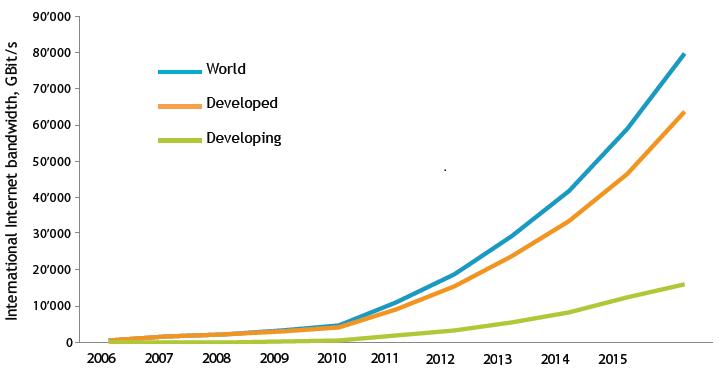
\includegraphics[width=5.0in,height=2.58in]{./media/image1.png}\caption{International internet bandwidth.}
	\end{Center}
\end{figure}
%%%%%%%%%%%%%%%%%%%% Figure/Image No: 1 Ends here %%%%%%%%%%%%%%%%%%%%

All figures, tables, etc. must have a caption, centre-justified in 11 pt. Times New Roman. Captions precede tables but follow figures.  Tables and figures must appear as close to their point of reference as satisfactory formatting of the final document permits.

\subsection{Acknowledgements}
(unnumbered) acknowledgements section may be inserted if required.
\subsection{References}
References should be cited in the main text.  The full references should be given as below (essentially IEEE format), in the order in which they are cited, in 10 pt. Times New Roman, with a 6pt spacing between each \cite{[1]}.

\section{Conclusions}
Papers in this format must not exceed twenty (16) pages in length. Papers should be submitted to the online submission site (https://www.ejmanager.com/my/jjcit/). Papers for initial consideration may be submitted in either .doc or .pdf format. Final, camera-ready versions should take into account referees’ suggested amendments.
\section*{Acknowledgements}
The authors would like to thank everyone, just everyone!

\begin{thebibliography}{99}
\bibitem{[1]} N. Szabo and R. Tanaka, Residue Arithmetic and Its Applications to Computer Technology. New York: McGraw Hill, 1967.
\bibitem{[2]}	J. Bajard, L. Didier and P. Kornerup, "An RNS Montgomery Modular Multiplication Algorithm," IEEE Trans. Computers, vol. 47, no. 7, pp. 766-776, July 1998.
\bibitem{[3]} 	J. Wolf and K. Pattipati, "A File Assignment Problem Model for Extended Local Area Network Environments," Proc. 10th Int'l conf. Distributed Computing Systems, pp. 221-230, 1990.
\bibitem{[4]}	J. O. Williams, Narrow-Band Analyzer, Ph.D. dissertation, Dept. Elect. Eng., Harvard Univ., Cambridge, MA, 1993.
\bibitem{[5]}	M. Kesler, "Highly Resonant Wireless Power Transfer in Subsea Applications," Colin McCarthy WiTricity Corporation, [Online], Available: http://www.witricity.com/assets/HRWPT-in-Subsea-Applications.pdf.
\bibitem{[6]}	M. Kesler, "Highly Resonant Wireless Power Transfer in Subsea Applications," Colin McCarthy WiTricity Corporation, [Online], Available: http://www.witricity.com/assets/HRWPT-in-Subsea-Applications.pdf.
\end{thebibliography}

\end{document}